\documentclass[11pt]{article}
\usepackage[english]{babel}
\usepackage[utf8]{inputenc}
\usepackage[dvipsnames]{xcolor}
\usepackage[most]{tcolorbox}
\usepackage[linguistics]{forest}
\usepackage{fancyhdr}
\usepackage{amsmath}
\usepackage{amssymb}
\usepackage{amsfonts}
\usepackage{amstext}
\usepackage{amsmath,amssymb,amsthm, thmtools}
\usepackage{tikz,lipsum,lmodern}
\usepackage{array}
\usepackage{lastpage}
\usepackage{multicol}
\usepackage{tikz-cd}
\usepackage{array}
\usepackage{dirtytalk}
\usepackage{qtree}
\usepackage{framed}
\usepackage[hyperfootnotes=false]{hyperref}
\hypersetup{
colorlinks=true,
linkcolor={mypink}}

\definecolor{mypink}{RGB}{255, 50, 147}
\definecolor{pink}{RGB}{255, 0, 147}

\setlength{\textheight}{9.3in}
\setlength{\topmargin}{-0.7in}
\setlength{\textwidth}{6.5in}
\setlength{\oddsidemargin}{0in}
\setlength{\evensidemargin}{0in}
\setlength{\parskip}{6pt}
\setlength{\parindent}{0pt}

\def\mbb{\mathbb}
\def\mb{\mathbf}
\def\mc{\mathcal}
\def\R{\mbb{R}}
\def\Q{\mbb{Q}}
\def\Z{\mbb{Z}}
\def\C{\mbb{C}}
\def\N{\mbb{N}}
\def\F{\mbb{F}}
\def\T{\mc{T}}
\def\A{\mc{A}}
\def\E{\mbb{E}}
\def\P{\mbb{P}}
\def\X{\mathfrak{X}}
\def\e{\epsilon}
\def\d{\delta}
\def\h{\hbar}
\def\w{\omega}
\def\l{\ell}
\def\Ra{\Rightarrow}
\def\La{\Leftarrow}
\def\and{\quad \text{and} \quad}
\def\la{\langle}
\def\ra{\rangle}
\def\n{\eta}
\def\sp{\vspace{3mm}}

\def\nemt{\neq \emptyset}
\newcommand{\dif}[2]{\frac{d#1}{d#2}}
\newcommand{\pardif}[2]{\frac{\partial #1}{\partial #2}}
\newcommand{\twopardif}[2]{\frac{\partial ^2 #1}{\partial #2^2}}
\newcommand{\Matrix}[1]{\begin{pmatrix} #1 \end{pmatrix}}
\newcommand{\Lint}[1]{\ointctrclockwise_{#1}}
\newcommand{\Ang}[1]{\left\langle #1 \right\rangle}
\newcommand{\Inn}{\langle \cdot , \cdot \rangle}
\newcommand{\norm}[1]{\left\| #1 \right\|}
\newcommand{\blanknorm}[1]{\| \cdot \|_{#1}}
\newcommand{\epfrac}[1]{\frac{\e}{#1}}
\newcommand{\ext}[1]{\tilde{\mb #1}}

\renewcommand{\epsilon}{\varepsilon}
\renewcommand{\bar}{\overline} 
\renewcommand{\hat}{\widehat}


\declaretheoremstyle[
  headfont=\color{mypink}\normalfont\bfseries,
%  bodyfont=\color{red}\normalfont\itshape,
]{pink}

\declaretheoremstyle[
  headfont=\color{black}\normalfont\bfseries,
%  bodyfont=\color{red}\normalfont\itshape,
]{boxedsolution}

\theoremstyle{pink}
\newtheorem{definition}{Definition}[section]

\theoremstyle{boxedsolution}
\newtheorem*{bproof}{Proof}
\newtheorem*{solution}{Solution}
  
\theoremstyle{definition}
\newtheorem{lemma}[definition]{Lemma}
\newtheorem{theorem}[definition]{Theorem}
\newtheorem{corollary}[definition]{Corollary}
\newtheorem{proposition}[definition]{Proposition}
\newtheorem{example}[definition]{Example}
\newtheorem{problem}{Problem}
\newtheorem{question}{Question}
\newtheorem{Goal}{Goal}

\newtheoremstyle{claim}
{\topsep}{\topsep}{}{}%              
{\bfseries}{:}%             
{5pt plus 1pt minus 1pt}{}%             
\theoremstyle{claim}
% change this to \newtheorem*{claim}{Claim} to leave things un-numbered
\newtheorem{claim}{Claim}



\newenvironment{boxsol}
    {\begin{framed}
    \begin{solution}
    }
    {
    \end{solution}    
    \end{framed}}
    
\newenvironment{boxproof}
    {\begin{framed}
    \begin{bproof}
    }
    {
    \end{bproof}    
    \end{framed}}

\pagestyle{fancy}
\fancyhf{}
\lhead{JCP421 - Assignment 2}
\rhead{Maxim Piatine (1005303100)}
\cfoot{Page \thepage \ of \pageref{LastPage}}

\begin{document}
\section*{Question 1}
Theoretically, the electron does orbit the proton and with the Schrodinger equation it still does; however, in a quantum mechanical way and not classical. Based on the figures presented, the hydrogen atom still has a revolving source around it but we can say does not depend on the angular momentum when $\l$ is equal to zero $(n,l,m)$.
\begin{center}
    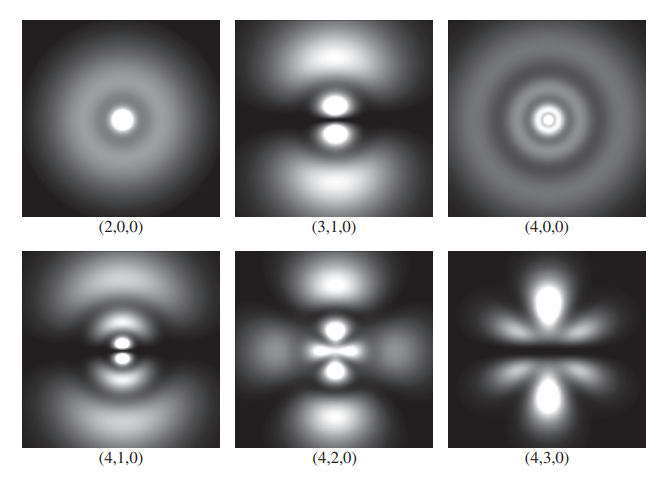
\includegraphics[width=12cm]{h.png}\\
    Source: David J. Griffiths, Introduction to Quantum Mechanics, 3rd ed.
\end{center}
An electron still has a wavelength, some movement, some mass, which means it also has a position and momentum. Therefore, there is a possibility for it to have angular momentum.\\
Also, the spherical harmonics for ground state $n=2$ and zero orbital angular momentum $\l = 0$ confirms my theory that the electron no longer depends on the angle.

\newpage
\section*{Question 2}
(a) $n = 2, s = 0$:
\[\la r|n,\l,m_\l\ra=\psi_{n,\l,m_\l}(\Vec{r})=R_{n\l}(r)Y^{m_\l}_\l(\theta, \phi)\]
\vspace{3mm}
\\The possible combinations for $n=2$:
\[\Big|n = 2,\l = 0,m_\l=0\Big\ra \text { } \text { , } \text { } \Big|n = 2,\l = 1,m_\l=1\Big\ra  \text { } \text { , } \text { }  \Big|n = 2,\l = 1,m_\l= -1\Big\ra  \text { } \text { , } \text { }  \Big|n = 2,\l = 1,m_\l=0\Big\ra\]

\vspace{3mm}

\[\la \Vec{r}| 2,0,0\ra = \psi_{200}(\Vec{r})=R_{2,0}Y^{0}_0=
\left(
\frac{1}{\sqrt{2}}a^{-3/2}\left(1-\frac{1}{2}\frac{r}{a}\right)e^{-r/2a}
\right)
\left(
\frac{1}{4}
\right)^{1/2}\]

\vspace{3mm}

\[\la \Vec{r}| 2,1,1\ra = \psi_{211}(\Vec{r})=R_{2,1}Y^{1}_1=
\left(
\frac{1}{2\sqrt{6}}a^{-3/2}\left(\frac{r}{a}\right)e^{-r/2a}
\right)
\left(
-\left(\frac{3}{8\pi}\right)^{1/2}\sin\theta e^{i\phi}
\right)\]


\vspace{3mm}

\[\la \Vec{r}| 2,1,-1\ra = \psi_{21-1}(\Vec{r})=R_{2,1}Y^{-1}_1=
\left(
\frac{1}{2\sqrt{6}}a^{-3/2}\left(\frac{r}{a}\right)e^{-r/2a}
\right)
\left(
\left(\frac{3}{8\pi}\right)^{1/2}\sin\theta e^{-i\phi}
\right)\]

\vspace{3mm}

\[\la \Vec{r}| 2,1,0\ra = \psi_{210}(\Vec{r})=R_{2,1}Y^{0}_1=
\left(
\frac{1}{2\sqrt{6}}a^{-3/2}\left(\frac{r}{a}\right)e^{-r/2a}
\right)
\left(
\left(\frac{3}{4\pi}\right)^{1/2}\cos\theta
\right)\]

\vspace{3mm}
The energy for all of these states corresponds to the energy level $n=2$:
\[E_{2} = -\left[\frac{m_e}{8\h^2}\left(\frac{e^2}{4\pi\e_0}\right)^2\right]\]


(b)
\[\delta H_{\l',m_\l',\l,m_\l}=\Matrix{
\la2,0,0|\delta H_{nc}|2,0,0\ra & \la2,0,0|\delta H_{nc}|2,1,1\ra & \la2,0,0|\delta H_{nc}|2,1,-1\ra & \la2,0,0|\delta H_{nc}|2,1,0\ra\\
\vspace{3mm}
\\\la2,1,1|\delta H_{nc}|2,0,0\ra & \la2,1,1|\delta H_{nc}|2,1,1\ra & \la2,1,1|\delta H_{nc}|2,1,-1\ra & \la2,1,1|\delta H_{nc}|2,1,0\ra\\
\vspace{3mm}
\\\la2,1,-1|\delta H_{nc}|2,0,0\ra & \la2,1,-1|\delta H_{nc}|2,1,1\ra & \la2,1,-1|\delta H_{nc}|2,1,-1\ra & \la2,1,-1|\delta H_{nc}|2,1,0\ra\\
\vspace{3mm}
\\\la2,1,0|\delta H_{nc}|2,0,0\ra & \la2,1,0|\delta H_{nc}|2,1,1\ra & \la2,1,0|\delta H_{nc}|2,1,-1\ra & \la2,1,0|\delta H_{nc}|2,1,0\ra\\
}\]


\newpage
\[\la2,0,0|\delta H_{nc}|2,0,0\ra = \la2,0,0| f(r)xy|2,0,0\ra=
\int^\infty_\infty\psi^*_{200}f(r)xy\psi_{200}d\tau \]
\vspace{3mm}
\[=\int^{2\pi}_0\int^{\pi}_0\int^\infty_0\psi^*_{200}f(r)xy\psi_{200}r^2\sin\theta dr d\phi d\theta=\int^{2\pi}_0\int^{\pi}_0\int^\infty_0\psi^*_{200}f(r)\sin\phi\cos\phi\sin^3\theta\psi_{200}r^4dr d\phi d\theta\]
\vspace{3mm}
\[=\int^{2\pi}_0\sin\phi\cos\phi d\phi
\int^{\pi}_0\sin^3\theta d\theta
\int^\infty_0\psi^*_{200}f(r)\psi_{200}r^4dr=0 \]


To save time and space, any term that contains only $\cos\phi\sin\phi$ in the $d\phi$ integral will equal zero. Let $\gamma$ be the constants and $r$ components to the specific radial wave functions of hydrogen and spherical harmonics:
\vspace{3mm}
\[\Big\la 2,1,0\Big|\delta H_{nc}\Big|2,0,0\Big\ra = \Big\la 2,0,0\Big|\delta H_{nc}\Big|2,1,0\Big\ra = \Big\la 2,1,1\Big|\delta H_{nc}\Big|2,1,1\Big\ra = \Big\la 2,1,-1\Big|\delta H_{nc}\Big|2,1,-1\Big\ra=\dots \]
\sp
\[\dots = \Big\la 2,1,0\Big|\delta H_{nc}\Big|2,1,0\Big\ra =0 \]
\sp
\[\Big\la 2,1,1\Big|\delta H_{nc}\Big|2,0,0\Big\ra=\int^{2\pi}_0e^{-i\phi}\sin\phi\cos\phi d\phi\int^\pi_0\sin^4\theta d\theta\gamma = 0 \]
Any integrals that contain $e^{-i\phi}\sin\phi\cos\phi d\phi$ is going to make the integral equal to zero:
\sp
\[\Big\la 2,0,0\Big|\delta H_{nc}\Big|2,1,-1\Big\ra = \Big\la 2,1,1\Big|\delta H_{nc}\Big|2,1,0\Big\ra = \Big\la 2,1,0\Big|\delta H_{nc}\Big|2,1,-1\Big\ra = 0\]
\sp
\[\Big\la 2,0,0\Big|\delta H_{nc}\Big|2,1,1\Big\ra=\int^{2\pi}_0e^{i\phi}\sin\phi\cos\phi d\phi\int^\pi_0\sin^4\theta d\theta\gamma = 0\]
Any integrals that contain $e^{-i\phi}\sin\phi\cos\phi d\phi$ is going to make the integral equal to zero:
\[\Big\la 2,1,-1\Big|\delta H_{nc}\Big|2,0,0\Big\ra=\Big\la 2,1,0\Big|\delta H_{nc}\Big|2,1,1\Big\ra=\Big\la 2,1,-1\Big|\delta H_{nc}\Big|2,1,0\Big\ra=0\]
\sp
The remaining two combinations:
\[\Big\la 2,1,-1\Big|\delta H_{nc}\Big|2,1,1\Big\ra=\int^{2\pi}_0e^{2i\phi}\sin\phi\cos\phi d\phi\int^{\pi}_0\sin^5\theta d\theta\gamma=\frac{8i\pi}{15}\gamma\]
\sp
\[\Big\la 2,1,1\Big|\delta H_{nc}\Big|2,1,-1\Big\ra=\int^{2\pi}_0e^{-2i\phi}\sin\phi\cos\phi d\phi\int^{\pi}_0\sin^5\theta d\theta\gamma=-\frac{8i\pi}{15}\gamma\]




\newpage
\[\delta H_{\l',m_\l',\l,m_\l}=\Matrix{
0 & 0 & 0 & 0\\
0 & 0 & -\frac{8\pi i}{15}\gamma & 0\\
0 & \frac{8\pi i}{15}\gamma & 0 & 0\\
0 & 0 & 0 & 0
}=\frac{8\pi i}{15}\gamma\Matrix{
0 & 0 & 0 & 0\\
0 & 0 & -1 & 0\\
0 & 1 & 0 & 0\\
0 & 0 & 0 & 0
}\]

(c) eigenvalues:
\[\left|\delta H_{nc}-E_r^{(1)}I\right|=0\]
\sp
\[=det\Matrix{
-E_r^{(1)} & 0 & 0 & 0\\
0 & -E_r^{(1)} & -1 & 0\\
0 & 1 & -E_r^{(1)} & 0\\
0 & 0 & 0 & -E_r^{(1)}}=-E_r^{(1)}\begin{vmatrix}
-E_r^{(1)} & -1 & 0\\
1 & -E_r^{(1)} & 0\\
0 & 0 & -E_r^{(1)}
\end{vmatrix}\]
\sp
\[=-E_r^{(1)}\left(0-0-E_r^{(1)}\begin{vmatrix}
-E_r^{(1)} & -1\\
1 & -E_r^{(1)}
\end{vmatrix}\right)=-E_r^{(1)}\left[-E_r^{(1)}\left(\left(-E_r^{(1)}\right)^2+1\right)\right]\]
\sp
\[=\left(E_r^{(1)}\right)^2\left(\left(E_r^{(1)}\right)^2+1\right)=0\]
\sp
\[E_{r_1}^{(1)} = 0 \text{ } \text{ , } \text{ } E_{r_2}^{(1)} = 0 \text{ } \text{ , } \text{ } E_{r_3}^{(1)} = -i \text{ } \text{ , } \text{ } E_{r_4}^{(1)} = i\]
\sp
\[\gamma = -\int^{\infty}_0 \left(\frac{1}{2\sqrt{6}}a^{-3/2}\left(\frac{r}{a}\right)e^{-r/2a}\right)^2
\left(\frac{3}{8\pi}\right)f(r)r^4dr=-\left(\frac{1}{64\pi a^5}\right)\int^\infty_0e^{-r/a}f(r)r^6dr\]
\sp
\[=-\left(\frac{1}{64\pi a^5}\right)\n\]
\sp
\\The first order corrections are:
\[E_1^{(1)} = 0\]
\sp
\[E_2^{(1)} = 0\]
\sp
\[E_3^{(1)} = -i\left(\frac{8\pi i}{15}\gamma\right)=i\left(\frac{8\pi i}{15}\right)\left(\frac{\n}{64\pi a^5}\right)=-\frac{\n}{120a^5}\]
\sp
\[E_4^{(1)} = i\left(\frac{8\pi i}{15}\gamma\right)=-i\left(\frac{8\pi i}{15}\right)\left(\frac{\n}{64\pi a^5}\right)=\frac{\n}{120a^5}\]
\newpage
(d) Since we found two eigenvalues that equate to zero, we know those two eigenvalues remove degeneracy; however, the states with non-zero eigenvalues still have degeneracies left. Therefore, the degeneracy only partially broke.
\begin{center}
    \begin{tikzpicture}
    \draw[black, thick, ->] (0,0) -- (0,5);
    \draw[black, thick, ->] (0,0) -- (10,0);
    \filldraw[black] (0,2.5) node[anchor=east]{$E$};
    \filldraw[black] (2.5,0) node[anchor=north]{$\l=0$};
    \filldraw[black] (7.5,0) node[anchor=north]{$\l=1$};
    \draw[black, thick] (1,2.5) -- (4,2.5);
    \filldraw[black] (2.5,2.5) node[anchor=south]{$E_2$};
    \draw[black, thick] (6,2.5) -- (9,2.5);
    \filldraw[black] (7.5,2.5) node[anchor=south]{$E_2$};
    \draw[black, thick] (6,4) -- (9,4);
    \filldraw[black] (7.5,4) node[anchor=south]{$E_2+\frac{\n}{120a^5}$};
    \draw[black, thick] (6,1) -- (9,1);
    \filldraw[black] (7.5,1) node[anchor=south]{$E_2-\frac{\n}{120a^5}$};
\end{tikzpicture}
\end{center}


\newpage
\section*{Question 3}
(a)
\[E_{\text{so}}^{(1)}(n,j,\l,s=1/2)=\frac{\left(E_n^{(0)}\right)^2}{m_ec^2}\Bigg\{\frac{n\left[j(j+1)-\l(\l+1)-3/4\right]}{\l(\l+1/2)(\l+1)}\Bigg\}=\frac{1}{2}hc\xi_{n,l}\left[j(j+1)-\l(\l+1)-3/4\right]\]
\vspace{5mm}
\[
n=2 \text{ } \text{ , } \text{ } \l=1 \text{ } \text{ , } \text{ } j = \frac{1}{2}  \text{ } \text{ , } \text{ } m_j = \pm\frac{1}{2} \text{ } \text{ , } \text{ } m_s = \pm \frac{1}{2} \text{ } \text{ , } \text{ } m_\l = \{-1,0,1\} \text{ } \text{ , } \text{ } m_\l = \{-1/2 , 1/2\}
\]
\vspace{3mm}
\[
n=2 \text{ } \text{ , } \text{ } \l=1 \text{ } \text{ , } \text{ } j = \frac{3}{2}  \text{ } \text{ , } \text{ } m_j = \pm\frac{3}{2}, \pm\frac{1}{2} \text{ } \text{ , } \text{ } m_s = \pm \frac{1}{2} \text{ } \text{ , } \text{ } m_\l = \{-1,0,1\} \text{ } \text{ , } \text{ } m_\l = \{-1/2 , 1/2\}
\]
\vspace{5mm}
\begin{center}
    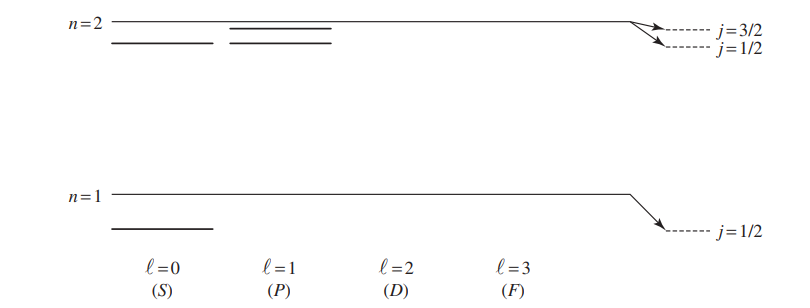
\includegraphics[width=15cm]{Screenshot 2022-02-16 191354.png}
\end{center}
\[
=\begin{cases}
|\phi_1\ra = |n=2 , \l = 1, m_\l = -1, m_s = -1/2\ra\\
|\phi_2\ra = |n=2 , \l = 1, m_\l = -1, m_s = 1/2\ra\\
|\phi_3\ra = |n=2 , \l = 1, m_\l = 0, m_s = -1/2\ra\\
|\phi_4\ra = |n=2 , \l = 1, m_\l = 0, m_s = 1/2\ra\\
|\phi_5\ra = |n=2 , \l = 1, m_\l = 1, m_s = -1/2\ra\\
|\phi_6\ra = |n=2 , \l = 1, m_\l = 1, m_s = 1/2\ra
\end{cases}
\]
\vspace{3mm}
\\(b)
\[\hat{L}\cdot\hat{S} = \frac{1}{2}\left(\hat{L}_+\hat{S}_-+\hat{L}_-\hat{S}_+\right)+\hat{L}_z\hat{S}_z\]
\vspace{3mm}
\[\left(\hat{L}\cdot\hat{S}\right)|\phi_n\ra = \left(\frac{1}{2}\left(\hat{L}_+\hat{S}_-+\hat{L}_-\hat{S}_+\right)+\hat{L}_z\hat{S}_z\right)\Big|\phi_n\Big\ra = \left(\frac{1}{2}\hat{L}_+\hat{S}_-\right)\Big|\phi_n\Big\ra + \left(\frac{1}{2}\hat{L}_-\hat{S}_+\right)\Big|\phi_n\Big\ra + \left(\hat{L}_z\hat{S}_z\right)\Big|\phi_n\Big\ra\]
\newpage
Using notes from tutorial sheet 3,
\[\hat{L}_\pm|n,\l,m_\l,s,m_s\ra = \h\sqrt{(\l\mp m_\l)(\l\pm m_\l + 1)}|n,\l,m_\l\pm 1,s,m_s\ra\]
\vspace{3mm}
\[\hat{S}_\pm|n,\l,m_\l,s,m_s\ra = \h\sqrt{(s\mp m_s)(s\pm m_s + 1)}|n,\l,m_\l,s,m_s\pm1\ra\]
\vspace{3mm}
\[\hat{L}_z|n,\l,m_\l,s,m_s\ra = \h m_\l|n,\l,m_\l,s,m_s\ra\]
\vspace{3mm}
\[\hat{S}_z|n,\l,m_\l,s,m_s\ra = \h m_s|n,\l,m_\l,s,m_s\ra\]
\vspace{3mm}
Using these eigenvalues to solve $\hat{L}\cdot\hat{S}|\phi\ra$:
\[\frac{1}{2}\hat{L}_+\hat{S}_-|m_\l,m_s\rangle = \frac{1}{2}\hbar\sqrt{(\ell- m_\ell)(\ell+ m_\ell + 1)}\h\sqrt{(s+ m_s)(s- m_s + 1)}|m_\l+1,m_s-1\rangle\]
\vspace{3mm}
\[=\frac{1}{2}\h^2\sqrt{(\ell- m_\ell)(\ell+ m_\ell + 1)(s+ m_s)(s- m_s + 1)}\Big|m_\l+1,m_s-1\Big\rangle\]
\vspace{3mm}
\[\frac{1}{2}\hat{L}_-\hat{S}_+|m_\l,m_s\rangle = \frac{1}{2}\h^2\sqrt{(\ell+ m_\ell)(\ell- m_\ell + 1)(s- m_s)(s+ m_s + 1)}\Big|m_\l-1,m_s+1\Big\rangle\]
\vspace{3mm}
\[
\hat{L}_z\hat{S}_z|m_\l,m_s\ra = \h m_\l \h m_s|m_\l,m_s\ra = \h^2 m_\l m_s|m_\l,m_s\ra
\]
\vspace{3mm}
\\Summing everything together:
\[\hat{L}\cdot\hat{S}|m_\l,m_s\ra = \frac{1}{2}\h^2\sqrt{(\ell- m_\ell)(\ell+ m_\ell + 1)(s+ m_s)(s- m_s + 1)}\Big|m_\l+1,m_s-1\Big\rangle + \dots \]
\vspace{3mm}
\[\dots + \frac{1}{2}\h^2\sqrt{(\ell+ m_\ell)(\ell- m_\ell + 1)(s- m_s)(s+ m_s + 1)}\Big|m_\l-1,m_s+1\Big\rangle + \dots\]
\vspace{3mm}
\[
\dots + \h^2 m_\l m_s|m_\l,m_s\ra
\]
\newpage
All the cases from part (a), plugging in $\l = 1 , m_\l = \{-1,0,1\}, s=\frac{1}{2}, m_s=\{-\frac{1}{2},\frac{1}{2}\}$
\[
= 
\begin{cases}
%1
\hat{L}\cdot\hat{S}\Big|m_\l=-1,m_s=-\frac{1}{2}\Big\ra= \hat{L}\cdot\hat{S}\Big|\phi_1\Big\ra
=\frac{\h^2}{2}\Big|-1,-\frac{1}{2}\Big\ra=\frac{\h^2}{2}\Big|\phi_1\Big\ra\\
\vspace{2mm}
%2
\\\hat{L}\cdot\hat{S}\Big|m_\l=-1,m_s=\frac{1}{2}\Big\ra = \hat{L}\cdot\hat{S}\Big|\phi_2\Big\ra
= \frac{\sqrt{2}}{2}\h^2\Big|0,\frac{-1}{2}\Big\ra-\frac{\h^2}{2}\Big|-1,\frac{1}{2}\Big\ra =\frac{\sqrt{2}}{2}\h^2\Big|\phi_3\Big\ra-\frac{\h^2}{2}\Big|\phi_2\Big\ra\\
\vspace{2mm}
%3
\\ \hat{L}\cdot\hat{S}\Big|m_\l=0,m_s=-\frac{1}{2}\Big\ra = \hat{L}\cdot\hat{S}\Big|\phi_3\Big\ra=
\frac{\sqrt{2}}{2}\h^2\Big|-1,\frac{1}{2}\Big\ra = \frac{\sqrt{2}}{2}\h^2\Big|\phi_2\Big\ra\\
\vspace{2mm}
%4
\\ \hat{L}\cdot\hat{S}\Big|m_\l=0,m_s=\frac{1}{2}\Big\ra = \hat{L}\cdot\hat{S}\Big|\phi_4\Big\ra=
\frac{\sqrt{2}}{2}\h^2\Big|1,\frac{-1}{2}\Big\ra = \frac{\sqrt{2}}{2}\h^2\Big|\phi_5\Big\ra \\
\vspace{2mm}
%5
\\\hat{L}\cdot\hat{S}\Big|m_\l=1,m_s=-\frac{1}{2}\Big\ra= \hat{L}\cdot\hat{S}\Big|\phi_5\Big\ra=
\frac{\sqrt{2}}{2}\h^2\Big|0,\frac{1}{2}\Big\ra - \frac{\h^2}{2}|1,\frac{-1}{2}\Big\ra=
\frac{\sqrt{2}}{2}\h^2\Big|\phi_4\Big\ra - \frac{\h^2}{2}|\phi_5\Big\ra\\
\vspace{2mm}
%5
\\\hat{L}\cdot\hat{S}\Big|m_\l=1,m_s=\frac{1}{2}\Big\ra = \hat{L}\cdot\hat{S}\Big|\phi_6\Big\ra=
\frac{\h^2}{2}\Big|1,\frac{1}{2}\Big\ra=\frac{\h^2}{2}\Big|\phi_6\Big\ra\\
\end{cases}
\]
\vspace{5mm}
\\(c) To save some time and space, every coordinate on the matrix is represented by\\ $\Big\la m'_\l,m'_s\Big|\hat{L}\cdot\hat{S}\Big|m_\l,m_s\Big\ra$. For each coordinate replace is $m_\l$ and $m_s$ accordingly like:\\ $\Big\la \phi_1\Big|\hat{L}\cdot\hat{S}\Big|\phi_1\Big\ra = \Big\la -1,\frac{-1}{2}\Big|\hat{L}\cdot\hat{S}\Big|-1,\frac{-1}{2}\Big\ra$
\[=\frac{hc\xi_{n,\l}}{\h^2}
\Matrix{
\Big\la\phi_1\Big|\hat{L}\cdot\hat{S}\Big|\phi_1\Big\ra & 0 & 0 & 0 & 0 & 0\\
\vspace{1mm}
\\0 & \Big\la\phi_2\Big|\hat{L}\cdot\hat{S}\Big|\phi_2\Big\ra & \Big\la\phi_2\Big|\hat{L}\cdot\hat{S}\Big|\phi_3\Big\ra & 0 & 0 & 0\\
\vspace{1mm}
\\0 & \Big\la\phi_3\Big|\hat{L}\cdot\hat{S}\Big|\phi_2\Big\ra & 0 & 0 & 0 & 0\\
\vspace{1mm}
\\0 & 0 & 0 & 0 & \Big\la\phi_4\Big|\hat{L}\cdot\hat{S}\Big|\phi_5\Big\ra & 0\\
\vspace{1mm}
\\0 & 0 & 0 & \Big\la\phi_5\Big|\hat{L}\cdot\hat{S}\Big|\phi_4\Big\ra & \Big\la\phi_5\Big|\hat{L}\cdot\hat{S}\Big|\phi_5\Big\ra  & 0\\
\vspace{1mm}
\\0 & 0 & 0 & 0 & 0 & \Big\la\phi_6\Big|\hat{L}\cdot\hat{S}\Big|\phi_6\Big\ra}\]


\newpage


\[=\frac{hc\xi_{n,\l}}{\h^2}
\Matrix{
\frac{\h^2}{2} & 0 & 0 & 0 & 0 & 0\\
\vspace{1mm}
\\0 & -\frac{\h^2}{2} & \frac{\sqrt{2}}{2}\h^2 & 0 & 0 & 0\\
\vspace{1mm}
\\0 & \frac{\sqrt{2}}{2}\h^2 & 0 & 0 & 0 & 0\\
\vspace{1mm}
\\0 & 0 & 0 & 0 & \frac{\sqrt{2}}{2}\h^2 & 0\\
\vspace{1mm}
\\0 & 0 & 0 & \frac{\sqrt{2}}{2}\h^2 & -\frac{\h^2}{2} & 0\\
\vspace{1mm}
\\0 & 0 & 0 & 0 & 0 & \frac{\h^2}{2}}\]
(d) After diagonalizing the matrix:
\[=hc\xi_{n,\l}
\Matrix{
-1 & 0 & 0 & 0 & 0 & 0\\
\vspace{1mm}
\\0 & -1 & 0 & 0 & 0 & 0\\
\vspace{1mm}
\\0 & 0 & \frac{1}{2} & 0 & 0 & 0\\
\vspace{1mm}
\\0 & 0 & 0 & \frac{1}{2} & 0 & 0\\
\vspace{1mm}
\\0 & 0 & 0 & 0 & \frac{1}{2} & 0\\
\vspace{1mm}
\\0 & 0 & 0 & 0 & 0 & \frac{1}{2}}\]
Using the diagram from part (a), we know all the constants that need to be used for equation (2):\\
Use $j=1/2$:
\sp
\[E^{(1)}_{so}\left(n=2,j=\frac{1}{2}, \l=1, s=\frac{1}{2}\right)=\frac{1}{2}hc\xi_{n,\l}\left[\frac{1}{2}\left(\frac{1}{2}+1\right)-1(1+1)-3/4\right]=-hc\xi_{n,\l}\]
\sp
\\Use $j=3/2$:
\[E^{(1)}_{so}\left(n=2,j=\frac{3}{2}, \l=1, s=\frac{1}{2}\right)=\frac{1}{2}hc\xi_{n,\l}\left[\frac{3}{2}\left(\frac{3}{2}+1\right)-1(1+1)-3/4\right]=\frac{1}{2}hc\xi_{n,\l}\]
The "good" basis states:
\[=\Matrix{
0 & 0 & 0 & 0 & 0 & 1\\
0 & -\sqrt{2} & 0 & 0 & \frac{1}{\sqrt{2}} & 0\\
0 & 1 & 0 & 0 & 1 & 0\\
-\frac{1}{\sqrt{2}} & 0 & 0 & \sqrt{2} & 0 & 0\\
1 & 0 & 0 & 1 & 0 & 0\\
0 & 0 & 1 & 0 & 0 & 0\\
}\]


\end{document}
